\documentclass{article}

\usepackage{fontspec}

\usepackage[backend=biber]{biblatex}
\addbibresource{literatur.bib}


\usepackage{codeanatomy}
\usepackage{listings}
\lstset {
     basicstyle=\small\ttfamily%
    ,language=%
    ,escapeinside={!}{!}%
    ,resetmargins=true%
    ,columns=flexible%
    ,literate={-}{-}1%
    ,keepspaces=true
}


%\usepackage{filecontents}
% command from ltxdoc
\newcommand{\pkg}[1]{\textsf{#1}}
% others shortcuts
\newcommand{\slsh}{\textbackslash{}}
\newcommand{\TikZ}{Ti\textit{k}Z}
\newcommand{\inputlisting}[1]{%
\lstinputlisting[%
    basicstyle=\footnotesize\ttfamily%
    ,xleftmargin=-40pt%
    ,resetmargins=true%
    ,firstline=5%
    ,language=%
    ,columns=flexible%
    ,escapeinside={}{}%
  ]{#1}%
}
%\def\thinmargin{\list{}{\rightmargin-30pt\leftmargin-40pt}\item[]}
%\let\endthinmargin=\endlist
\newenvironment{thinmargin}{}{}

\usepackage{readprov}     % need for \GetFileInfo{}
\usepackage{hyperref}

\title{
  \pkg{codeanatomy} -- Draw Code Anatomy%
  \thanks{This file describes \fileversion,
    last revised \filedate.}\\\vspace*{2ex}
  \normalsize{Usage with \pkg{listings}}
}

\author{
 Hồng-Phúc Bùi%
 \thanks{
   E-mail:
   \href{mailto:Hồng-Phúc Bùi}
     {hong-phuc.bui (at) htwsaar dot de}
  }
}

\date{Released \filedate}



\begin{document}

\GetFileInfo{codeanatomy.sty}

\maketitle
\tableofcontents


\section{General Usage with Package \pkg{listings}}
\subsection{Setup Package \pkg{listings}}
The most important setup for the package \pkg{listings} is the delimiter to escape \LaTeX{}
commands in Listing. With this escape delimiter we can mark a piece of code as with \verb|\cPart|.
In this example we use \verb|!| and \verb|!| as delimiter. Code between \verb|!| and \verb|!| is evaluated as
\LaTeX{}-code.

\lstset {
    escapeinside={+}{+}
}
\begin{thinmargin}
\begin{tikzpicture}[remember picture,overlay]
% {[on background layer]\draw[code grid debug] (-3.5,-0.5) grid (5.5,4.5);}
\node(code) [anatomy] at (0,0){%
\begin{lstlisting}
\usepackage{codeanatomy}
\usepackage{listings}
\lstset {
   basicstyle=\small\ttfamily
  ,escapeinside=+\cPart{delimiter}{\{!\}\{!\}}+
}
\end{lstlisting}
};%

\codeAnnotation{delimiterText} (4,-0.5) {Setup \texttt{!} and \texttt{!}\\as delimiter}

\draw[->, annotation] (delimiterText) -- (pic cs:delimiter);
\end{tikzpicture}
\end{thinmargin}


Delimiter can also be reset in \verb|document|-Environment, typical just before a new \verb:\begin{lstlisting}:
environment so each anatomy can have different delimiter. The fact is, in this document I use \verb|+| and \verb|+| for
the above listing, so that I can typeset \verb|!| in this listing.

You may also want to set option \verb|keepspaces| to \verb|true|, sothat your reader can easy copy past
your example code.

\subsection{Typeset Code}
% -----------------------
The command \verb|\codeBlock| does not work if the environment \verb|lstlisting| is passed to its argument. So instead of
\verb|\codeBlock| we must use the \TikZ{} command \verb|\node|:

\begin{thinmargin}
\begin{tikzpicture}[remember picture]
\node(code) [anatomy] at (0,0) {
\begin{lstlisting}
\begin{tikzpicture}[remember picture]
+\cPart{tikzNode}{\slsh{}node(code) [anatomy] at (0,0)}+ {
+\cPart{listingBegin}{\texttt{\slsh{}begin\{lstlisting\}}}\vspace{1.5pt}+
+\mtPoint{mostLeft}+function gcd(p,q) {
    if (q === 0) {
        return q;
    }else{
        let r = p % q;
        return gcd(q, r);+\extremPoint{mostRight}+
    }
}+\mbPoint{mostBottom}+
+\cPart{listingEnd}{\texttt{\slsh{}end\{lstlisting\}}}+
}+\cPart{semiColon}{;}+
\end{tikzpicture}
\end{lstlisting}
};

\fitExtrem{listingContent}{(mostLeft) (mostRight) (mostBottom)}

% Annotations
\codeAnnotation{tikzNodeText} (-2, 5.5)      {use \texttt{\slsh{}node}\\instead of\\\texttt{\slsh{}codeBlock}}
\codeAnnotation{listingText}  (-2, 3)        {typeset code\\in\\\texttt{lstlisting}\\environment}
\codeAnnotation{listingContentText} (6.5, 3) {whitespaces\\in code\\are kept}
\codeAnnotation{semiColonText} (6.5, 0.6)    {don't forget\\semicolon}

% Arrows from labels to code parts
\draw[->,annotation] (tikzNodeText)       -- (pic cs:tikzNode.west);
\draw[->,annotation] (listingText)        -- (pic cs:listingBegin.west);
\draw[->,annotation] (listingText)        -- (pic cs:listingEnd.west);
\draw[->,annotation] (listingContentText) -- (pic cs:listingContent);
\draw[->,annotation] (semiColonText)      -- (pic cs:semiColon);
\end{tikzpicture}
\end{thinmargin}

Figure~\ref{fig:full-formatted-code} shows result of the above code.

\begin{figure}[ht]
\centering
\begin{tikzpicture}[remember picture]
\node(code) [anatomy] at (0,0) {
\begin{lstlisting}
function gcd(p,q) {
    if (q === 0) {
        return q;
    }else{
        let r = p % q;
        return gcd(q, r)
    }
}
\end{lstlisting}
};
\end{tikzpicture}
\caption{Code Listing is formatted\label{fig:full-formatted-code}}
\end{figure}

\subsection{Mark Code}
% --------------------

The command \verb|\cPart| can be used to mark single-line code parts. For
multiple-line code parts once can use \verb|\xxxPoint| family to mark the outer most
points of code parts and \verb|\fitExtrem| to cover exterm points of a code part.
These commmands must be put between escape delimiter, here \verb|!| and \verb|!|.

\begin{thinmargin}
\begin{tikzpicture}[remember picture]
\node(code) [anatomy] at (0,0) {
\begin{lstlisting}
\begin{tikzpicture}[remember picture]
\node(code) [anatomy] at (0,0) {
+\texttt{\slsh{}begin\{lstlisting\}}+
!\cPart{fnHead}{function \cPart{fnName}{gcd} \cPart{paramList}{(p,q)}}! {
    +\cPart{ep1}{!\slsh{}mtPoint\{mostLeft\}!}+if (q === 0) {
        return q;
    }else{
        +\cPart{cp}{!\slsh{}cPart\{localVar\}\{let r\}!}+ = p % q;
        return gcd(q, r);+\cPart{ep2}{!\slsh{}extremPoint\{mostRight\}!}+
    }+\cPart{ep3}{!\slsh{}mbPoint\{mostBottom\}!}+
}
+\texttt{\slsh{}end\{lstlisting\}}+
};
\fitExtrem{fnBody}{(mostLeft) (mostRight) (mostBottom)}
\end{tikzpicture}
\end{lstlisting}
};
% Annotations
\codeAnnotation{epText} (12,2.75) {xxx\texttt{Point}-s mark\\outer most\\of the function body}
\codeAnnotation{cpText} (-2,3) {\texttt{cPart} marks a\\single line\\code part}
% Arrows
\draw[->,annotation] (epText) -- (ep1.south east);
\draw[->,annotation] (epText) -- (ep2.east);
\draw[->,annotation] (epText) -- (ep3.south east);
\draw[->,annotation] (cpText) -- (cp);
\end{tikzpicture}
\end{thinmargin}

Figure~\ref{fig:listing-code-parts} shows the result of the above code.

\begin{figure}[ht]
\centering
\lstset{escapeinside={!}{!}}
\begin{tikzpicture}[remember picture]
\node(code) [anatomy] at (0,0) {
\begin{lstlisting}
!\cPart{fnHead}{function \cPart{fnName}{gcd}\cPart{paramList}{(p,q)}}! {
    !\mtPoint{mostLeft}!if (q === 0) {
        return q;
    }else{
        !\cPart{localVar}{let r}! = p % q;
        return gcd(q, r);!\extremPoint{mostRight}!
    }!\mbPoint{mostBottom}!
}
\end{lstlisting}
};
\fitExtrem{fnBody}{(mostLeft) (mostRight) (mostBottom)}
\end{tikzpicture}
\caption{Code Listing with mark of code parts\label{fig:listing-code-parts}}
\end{figure}


\subsection{Highlight some tokens}

\begin{filecontents}{recursive-with-bug.tex}
\lstset{escapeinside={!}{!},basicstyle=\linespread{1.8}}
\begin{tikzpicture}[remember picture]
\tikzstyle{token} = [code part, fill=yellow]
\tikzstyle{bug} = [code part, fill=red!50]
\node(code) [anatomy] at (0,0) {
\begin{lstlisting}
function !\cPart[token]{fnName}{gcd}! (p,q) {
    if (q === 0) {
        return !\cPart[bug]{bug}{q}!;
    } else {
        let r = p % q;
        return !\cPart[token]{recursive}{gcd}!(q, r);
    }
}
\end{lstlisting}
};
\codeAnnotation{recursiveText}    (-1,2) {Function can\\call itself.}
\codeAnnotation{bugText}         ( 5,2.25) {This is\\the bug.}

\draw[->, annotation] (recursiveText) to[out=50, in=190]  (pic cs:fnName);
\draw[->, annotation] (recursiveText) to[out=-20, in=175] (pic cs:recursive.north west);
\draw[->, annotation] (bugText)       to[out=190,in=-20]  (pic cs:bug.south east);
\end{tikzpicture}
\end{filecontents}

%\begin{thinmargin}
\inputlisting{recursive-with-bug.tex}
%\end{thinmargin}

\input{recursive-with-bug.tex}





\subsection{Add Annotations to Listing}
% -------------------------------------
This step is the same as the description in the usage document of package \pkg{codeanatomy}.
Readers can typeset annotations to the above listing like an exercise.




\section{Some examples}
% ====================

Most of examples in this section are redrawn from the textbook~\autocite{sedgewick-wayne-2016}.

\subsection{Anatomy of a Java Program~\autocite[5]{sedgewick-wayne-2016}}
% -----------------------------------

\begin{filecontents}{java-program.tex}
\lstset{escapeinside={!}{!}}
\begin{tikzpicture}[remember picture]
\node(code) [anatomy] at (0,0){%
\begin{lstlisting}
public !\iPart{class}{class}! !\cPart{className}{HelloWorld}!
{
    !\mtPoint{mainLeft}!public static void main(String[] argv)
    {
        !\hmtPoint{left}\iPart{assign}{
            \bgcode{// Prints "Hello World" in the terminal window}}
            \extremPoint{fnR} \extremPoint{mR}!
        !\iPart{fnCall}{System.out.print("Hello World");}\dmbPoint{mostBottom}!
    }!\mbPoint{mainBottom}!
}
\end{lstlisting}
};

\fitExtrem{classBody}{(mainLeft) (mR) (mainBottom)}
\fitExtrem{functionBody}{(left) (fnR) (mostBottom)}


\codeAnnotation{fileNameText} (1.5,5) {text file named \texttt{HelloWorld.java}}
\codeAnnotation{classNameText} (3.5,4.25) {name}
\codeAnnotation{classBodyText} (6.5,3.6) {\texttt{main()} method}
\codeAnnotation{functionBodyText} (2.5,-0.5) {body}
\codeAnnotation{statement} (8,0) {statements}

{[on background layer]
\draw[->,annotation] (fileNameText) -- (pic cs:class);
\draw[->,annotation] (classNameText) -- (pic cs:className);
\draw[->,annotation] (classBodyText.south west) -- (pic cs:classBody);
\draw[->,annotation] (functionBodyText) -- (pic cs:functionBody);
\draw[->,annotation] (statement) -- (pic cs:assign.353);
\draw[->,annotation] (statement) -- (pic cs:fnCall.350);
}
\end{tikzpicture}
\end{filecontents}

%\begin{thinmargin}
\inputlisting{java-program.tex}
%\end{thinmargin}

\lstset{escapeinside={!}{!}}
\begin{tikzpicture}[remember picture]
\node(code) [anatomy] at (0,0){%
\begin{lstlisting}
public !\iPart{class}{class}! !\cPart{className}{HelloWorld}!
{
    !\extremPoint{mainLeft}[most top]!public static void main(String[] argv)
    {
        !\extremPoint{left}[most top]\iPart{assign}{
          \bgcode{// Prints "Hello World" in the terminal window}}
          \extremPoint{fnR} \extremPoint{mR}!
        !\iPart{fnCall}{System.out.print( "Hello World");}\extremPoint{mostBottom}[most bottom]!
    }!\extremPoint{mainBottom}[most bottom]!
}
\end{lstlisting}
};

\fitExtrem{classBody}{(mainLeft) (mR) (mainBottom)}
\fitExtrem{functionBody}{(left) (fnR) (mostBottom)}


\codeAnnotation{fileNameText} (1.5,5) {text file named \texttt{HelloWorld.java}}
\codeAnnotation{classNameText} (3.5,4.25) {name}
\codeAnnotation{classBodyText} (6.5,3.6) {\texttt{main()} method}
\codeAnnotation{functionBodyText} (2.5,-0.5) {body}
\codeAnnotation{statement} (8,0) {statements}

\draw[->,annotation] (fileNameText) -- (class);
\draw[->,annotation] (classNameText) -- (className);
\draw[->,annotation] (classBodyText.south west) -- (classBody);
\draw[->,annotation] (functionBodyText) -- (functionBody);
\draw[->,annotation] (statement) -- (assign.353);
\draw[->,annotation] (statement) -- (fnCall.350);
\end{tikzpicture}


\subsection{Anatomy of an expression~\autocite[17]{sedgewick-wayne-2016}}
% -----------------------------------

\begin{filecontents}{java-expression.tex}
\lstset{escapeinside={!}{!}}
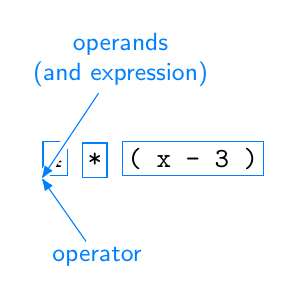
\begin{tikzpicture}[remember picture]
\codeBlock{\cPart{op1}{4} \cPart{op}{*} \cPart{op2}{( x - 3 )} }

\codeAnnotation{operand}  (1,1.5) {operands\\(and expression)}
\codeAnnotation{operator} (0.7,-1) {operator}

\draw[->,annotation] (operand) --  (pic cs:op1.north);
\draw[->,annotation] (operand) --  (pic cs:op2.north);
\draw[->,annotation] (operator) -- (pic cs:op.south);
\end{tikzpicture}
\end{filecontents}

\begin{thinmargin}
    \inputlisting{java-expression.tex}
\end{thinmargin}

\lstset{escapeinside={!}{!}}
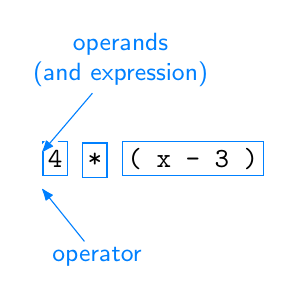
\begin{tikzpicture}[remember picture]    
\codeBlock{\cPart{op1}{4} \cPart{op}{*} \cPart{op2}{( x - 3 )} }

\codeAnnotation{operand}  (1,1.5) {operands\\(and expression)}
\codeAnnotation{operator} (0.7,-1) {operator}

\draw[->,annotation] (operand) -- (op1.north);
\draw[->,annotation] (operand) -- (op2.north);
\draw[->,annotation] (operator) -- (op.south);
\end{tikzpicture}


\subsection{Using a primitive Data Type~\autocite[17]{sedgewick-wayne-2016}}
% -------------------------------------

\begin{filecontents}{using-a-primitive-data-type.tex}
\lstset{escapeinside={!}{!}}
\begin{tikzpicture}[
     remember picture %
    ,code annotation/.append style = { % customize style of annotation text
        font=\sffamily\footnotesize
    }
]
{[on background layer]\draw[code grid debug] (-2.5,-0.5) grid (2.5,2.5);}
\node(code) [anatomy] at (0,0){%
\begin{lstlisting}
!\cPart{d}{int a, b;}!
!\iPart{v}{a}! = !\cPart{l}{1234}!;
!\iPart{a}{b = 99}!;
!\cPart{i}{int c = a + b}!;
\end{lstlisting}
};
% Annotations
\codeAnnotation{declareText}   (   1,2.75 )   {declaration statement}
\codeAnnotation{literalText}   (  2.5,1.45)   {literal}
\codeAnnotation{varText}       (-1.5,1.75 )   {variable name}
\codeAnnotation{assignText}    (-1.5,0.75 )   {assignment\\statement}
\codeAnnotation{initText}      (-1.5,-0.75)   {inline initialization\\statement}
% Arrows
\draw[->,annotation] (declareText) -- (pic cs:d);
\draw[->,annotation] (literalText) -- (pic cs:l);
\draw[->,annotation] (varText.south east) -- (pic cs:v);
\draw[->,annotation] (assignText) -- (pic cs:a);
\draw[->,annotation] (initText) -- (pic cs:i.south west);
\end{tikzpicture}
\end{filecontents}

\begin{thinmargin}
    \inputlisting{using-a-primitive-data-type.tex}
\end{thinmargin}

\input{using-a-primitive-data-type.tex}

\subsection{Anatomy of a method signature~\autocite[30]{sedgewick-wayne-2016}}
% ---------------------------------------

\begin{filecontents}{anatomy-of-a-method-signature.tex}
\lstset{escapeinside={!}{!}}
\begin{tikzpicture}[remember picture,overlay]
\node(code) [anatomy] at (0,0) {
\begin{lstlisting}
public class !\iPart{l}{Math}!
    ....
    !\cPart{s}{\bgcode{static} \iPart{r}{double} \iPart{n}{sqrt}(\iPart{a}{double} a)}!
    ....
\end{lstlisting}
};
% Annotation
\codeAnnotation{lText}    (3,2.5)   {library name}
\codeAnnotation{sText}   (-1,1)     {signature}
\codeAnnotation{nText}  (4.5,1.5)   {method name}
\codeAnnotation{rText}  (2.0,-0.51) {return type}
\codeAnnotation{aText}  (4.5,-0.51) {argument type}
% Arrows
\draw[->, annotation] (lText) -- (pic cs:l);
\draw[->, annotation] (nText) -- (pic cs:n);
\draw[->, annotation] (sText) -- (pic cs:s);
\draw[->, annotation] (rText) -- (pic cs:r);
\draw[->, annotation] (aText) -- (pic cs:a);
\end{tikzpicture}
\end{filecontents}

\begin{thinmargin}
    \inputlisting{anatomy-of-a-method-signature.tex}
\end{thinmargin}

\input{anatomy-of-a-method-signature.tex}

\subsection{Using a library method~\autocite[30]{sedgewick-wayne-2016}}
% --------------------------------

\begin{filecontents}{using-a-library-method.tex}
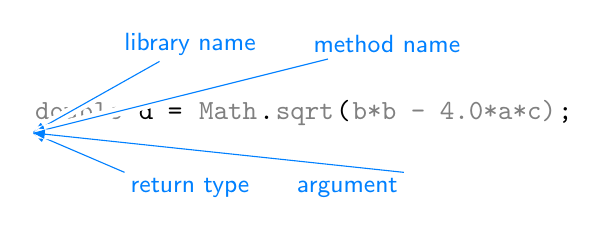
\begin{tikzpicture}[remember picture]
\codeBlock{%
\iPart{r}{double} d = \iPart{l}{Math}.\iPart{m}{sqrt}(\iPart{a}{b*b - 4.0*a*c)};
}
% Annotation
\codeAnnotation{lText}   (2, 1.125) {library name}
\codeAnnotation{mText} (4.5, 1.125) {method name}
\codeAnnotation{rText}   (2,-0.7)   {return type}
\codeAnnotation{aText}   (4,-0.7)   {argument}
% Arrows
\draw[->,annotation] (lText) -- (pic cs:l);
\draw[->,annotation] (mText) -- (pic cs:m);
\draw[->,annotation] (rText.north west) -- (pic cs:r);
\draw[->,annotation] (aText.north east) -- (pic cs:a);
\end{tikzpicture}
\end{filecontents}

\begin{thinmargin}
    \inputlisting{using-a-library-method.tex}
\end{thinmargin}

\input{using-a-library-method.tex}

\subsection{Anatomy of an \texttt{if} statement~\autocite[51]{sedgewick-wayne-2016}}
% ---------------------------------------------

\begin{filecontents}{anatomy-of-an-if-statement.tex}
\lstset{escapeinside={!}{!}}
\begin{tikzpicture}[remember picture]
%    {[on background layer]\draw[code grid debug] (-2.5,-0.5) grid (2.5,2.5);}
\node(code) [anatomy] at (0,0) {%
\begin{lstlisting}
if (!\cPart{e}{x > y}!)
{
    int t = x;!\mtPoint{tr}!
    x = y;
   !\mbPoint{bl}! y = t;!\extremPoint{br}!
}
\end{lstlisting}
};

\fitExtrem{b}{(tr) (bl) (br)}
% Annotation
\codeAnnotation{eText}  (1,3.5)  {boolean\\expression}
\codeAnnotation{bText} (-1,1.125)  {sequence\\of \extremPoint{bPoint}[0.75ex]\\statements}
% Arrow
\draw[->,annotation] (eText)  -- (pic cs:e);
\draw[->,annotation] (bPoint) -- (pic cs:b);
\end{tikzpicture}
\end{filecontents}

\begin{thinmargin}
    \inputlisting{anatomy-of-an-if-statement.tex}
\end{thinmargin}

\input{anatomy-of-an-if-statement.tex}

\subsection{Anatomy of a \texttt{while} loop~\autocite[54]{sedgewick-wayne-2016}}
% ------------------------------------------

\begin{filecontents}{anatomy-of-a-while-loop.tex}
\lstset{escapeinside={!}{!}}
\begin{tikzpicture}[remember picture]
%    {[on background layer]\draw[code grid debug] (-2.5,-0.5) grid (2.5,2.5);}
\node(code) [anatomy] at (0,0) {
\begin{lstlisting}
!\cPart{i}{\bgcode{int power = 1;}}\phantom{\rule[-2ex]{0.1ex}{0.1ex}}!
while ( !\cPart{c}{power <= n/2}! )
!\cPart{po}{\{}!
    !\cPart{b}{power = 2*power;}!
!\cPart{pc}{\}}!
\end{lstlisting}
};

% Annotation
\codeAnnotation{iText}  (-1,3.25) {initialization is a\\separate statement}
\codeAnnotation{cText} (3.5,3)    {loop-\\continuation\\condition}
\codeAnnotation{pText} (-1.5,0.5) {braces are\\optional\\when body\\is a single\\statement}
\codeAnnotation{bText} (2.125,-0.5) {body}
% Arrows
\draw[->,annotation] (iText) -- (pic cs:i.north west);
\draw[->,annotation] (cText) -- (pic cs:c);
\draw[->,annotation] (bText) -- (pic cs:b);
\draw[->,annotation] (pText) -- (pic cs:po);
\draw[->,annotation] (pText) -- (pic cs:pc);
\end{tikzpicture}
\end{filecontents}

\begin{thinmargin}
    \inputlisting{anatomy-of-a-while-loop.tex}
\end{thinmargin}


\input{anatomy-of-a-while-loop.tex}

\subsection{Anatomy of a \texttt{for} loop~\autocite[59]{sedgewick-wayne-2016}}
% ----------------------------------------

\begin{filecontents}{anatomy-of-a-for-loop.tex}
\lstset{escapeinside={!}{!}}
\begin{tikzpicture}[
     remember picture
    ,code annotation/.append style={%
        font=\sffamily\itshape\scriptsize
    }
]
    % {[on background layer]\draw[code grid debug] (-2.5,-0.5) grid (5.5,3.5);}
\node(code) [anatomy] at (0,0){%
\begin{lstlisting}
!\iPart{init}{\bgcode{int power = 1;}}!
for ( !\cPart{i}{int i = 0}!; !\cPart{c}{i <= n}!; !\cPart{u}{i++}! )
{
    !\mtPoint{left}!System.out.println(i + " " + power);!\mtPoint{right}!
    power *= 2;!\mbPoint{bottom}!
}
\end{lstlisting}
};
\fitExtrem{b}{(left) (right) (bottom)}
% Annotations
\codeAnnotation{initText} (-1.5,2.7)   {initialize another\\
                                        variable in a \extremPoint{initPoint}[0.75ex]\\
                                        separate\\statement}
\codeAnnotation{iText}       (1.2,3.5)   {declare and initialize\\
                                        a loop control variable}
\codeAnnotation{cText}     (3.5,3)     {loop-\\continuation\\condition}
\codeAnnotation{uText}       (6,3)     {increment}
\codeAnnotation{bText}     (3.5,-0.25) {body}
% arrows on the background
{[on background layer]
\draw[->,annotation] (initPoint) -- (pic cs:init.north west);
\draw[->,annotation] (iText) -- (pic cs:i);
\draw[->,annotation] (cText) -- (pic cs:c);
\draw[->,annotation] (uText) -- (pic cs:u);
\draw[->,annotation] (bText) -- (pic cs:b);
}
\end{tikzpicture}
\end{filecontents}

\begin{thinmargin}
    \inputlisting{anatomy-of-a-for-loop.tex}
\end{thinmargin}

\input{anatomy-of-a-for-loop.tex}

\subsection{Anatomy of a static method~\autocite[196]{sedgewick-wayne-2016}}
% ----------------------------------------
\begin{filecontents}{anatomy-of-a-static-method.tex}
\lstset{escapeinside={!}{!}}
\begin{tikzpicture}[remember picture]
    %{[on background layer]\draw[code grid debug] (-2.5,-0.5) grid (8.5,3.5);}
\node(code) [anatomy] at (0,0) {%
\begin{lstlisting}
!\cPart{s}{public static \cPart{rt}{double} \cPart{fn}{harmonic}(\cPart{al}{\iPart{at}{int} \iPart{pv}{n}})}!
{
    !\hmtPoint{left}\cPart{lv}{double sum}! = 0.0;
    for (int i = 0; i <= n; ++i)!\extremPoint{right}!
    {
        sum += 1.0/i;
    }
    !\cPart{rs}{return sum;}\dmbPoint{bottom}!
}
\end{lstlisting}
};

\fitExtrem{b}{(left) (right) (bottom)}

% Annotation
\codeAnnotation{sText}  (-0.7,5.25)  {signature}
\codeAnnotation{rtText}    (2,5.25)  {return\\type}
\codeAnnotation{fnText}  (  4,5.25)  {method\\name}
\codeAnnotation{alText}  (  6,5.25)  {argument\\list}
\codeAnnotation{atText} (6.75,1.75)  {argument\\type}
\codeAnnotation{pvText}  (7.5,2.70)  {parameter\\variable}
\codeAnnotation{lvText} (-0.7,3)     {local\\variable}
\codeAnnotation{bText}  (-0.7,1.5)   {method\\body}
\codeAnnotation{rsText}  (3,-0.4)    {return statement}
% Arrows
\draw[->,annotation] (sText) -- (pic cs:s.north west);
\draw[->,annotation] (rtText) -- (pic cs:rt);
\draw[->,annotation] (fnText) -- (pic cs:fn);
\draw[->,annotation] (alText) -- (pic cs:al);
\draw[->,annotation] (atText) -- (pic cs:at);
\draw[->,annotation] (pvText) -- (pic cs:pv);
\draw[->,annotation] (lvText) -- (pic cs:lv.west);
\draw[->,annotation] (bText) -- (pic cs:b);
\draw[->,annotation] (rsText) -- (pic cs:rs);
\end{tikzpicture}
\end{filecontents}

\begin{thinmargin}
    \inputlisting{anatomy-of-a-static-method.tex}
\end{thinmargin}

\input{anatomy-of-a-static-method.tex}


\printbibliography

\end{document}